%% Creator: Inkscape 1.2.2 (b0a8486541, 2022-12-01), www.inkscape.org
%% PDF/EPS/PS + LaTeX output extension by Johan Engelen, 2010
%% Accompanies image file '\assetPath /Images/InkscapeDemo/Acorn-RiscPC-LaTeX.pdf' (pdf, eps, ps)
%%
%% To include the image in your LaTeX document, write
%%   \input{<filename>.pdf_tex}
%%  instead of
%%   \includegraphics{<filename>.pdf}
%% To scale the image, write
%%   \def\svgwidth{<desired width>}
%%   \input{<filename>.pdf_tex}
%%  instead of
%%   \includegraphics[width=<desired width>]{<filename>.pdf}
%%
%% Images with a different path to the parent latex file can
%% be accessed with the `import' package (which may need to be
%% installed) using
%%   \usepackage{import}
%% in the preamble, and then including the image with
%%   \import{<path to file>}{<filename>.pdf_tex}
%% Alternatively, one can specify
%%   \graphicspath{{<path to file>/}}
%% 
%% For more information, please see info/svg-inkscape on CTAN:
%%   http://tug.ctan.org/tex-archive/info/svg-inkscape
%%
\begingroup%
  \makeatletter%
  \providecommand\color[2][]{%
    \errmessage{(Inkscape) Color is used for the text in Inkscape, but the package 'color.sty' is not loaded}%
    \renewcommand\color[2][]{}%
  }%
  \providecommand\transparent[1]{%
    \errmessage{(Inkscape) Transparency is used (non-zero) for the text in Inkscape, but the package 'transparent.sty' is not loaded}%
    \renewcommand\transparent[1]{}%
  }%
  \providecommand\rotatebox[2]{#2}%
  \newcommand*\fsize{\dimexpr\f@size pt\relax}%
  \newcommand*\lineheight[1]{\fontsize{\fsize}{#1\fsize}\selectfont}%
  \ifx\svgwidth\undefined%
    \setlength{\unitlength}{621.63151538bp}%
    \ifx\svgscale\undefined%
      \relax%
    \else%
      \setlength{\unitlength}{\unitlength * \real{\svgscale}}%
    \fi%
  \else%
    \setlength{\unitlength}{\svgwidth}%
  \fi%
  \global\let\svgwidth\undefined%
  \global\let\svgscale\undefined%
  \makeatother%
  \begin{picture}(1,1.11722135)%
    \lineheight{1}%
    \setlength\tabcolsep{0pt}%
    \put(0,0){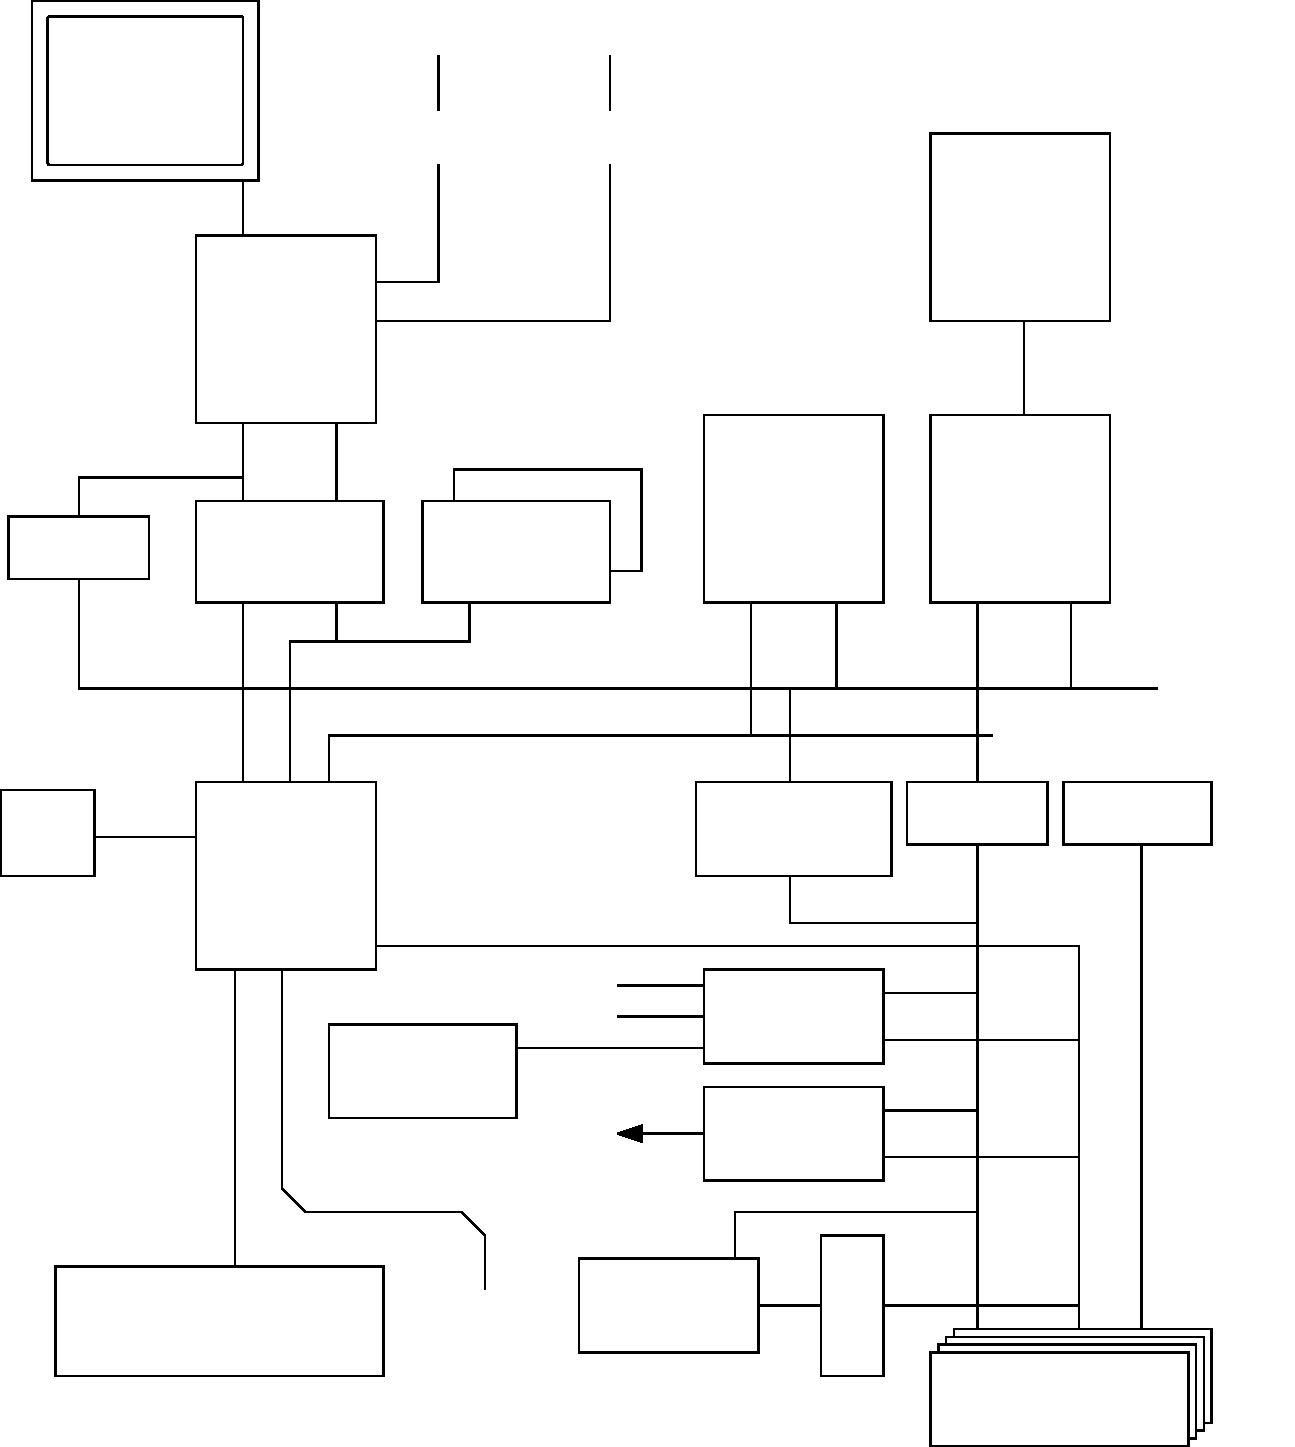
\includegraphics[width=\unitlength,page=1]{\assetPath /Images/InkscapeDemo/Acorn-RiscPC-LaTeX.pdf}}%
    \put(0.32635894,0.39271658){\color[rgb]{0,0,0}\makebox(0,0)[lt]{\lineheight{0}\smash{\begin{tabular}[t]{l}Lo 16-bit buffered I/O data\end{tabular}}}}%
    \put(0.19967617,0.94770774){\color[rgb]{0,0,0}\makebox(0,0)[lt]{\lineheight{0}\smash{\begin{tabular}[t]{l}video\end{tabular}}}}%
    \put(0.36218994,0.90107392){\color[rgb]{0,0,0}\makebox(0,0)[lt]{\lineheight{0}\smash{\begin{tabular}[t]{l}analogue\\sound\end{tabular}}}}%
    \put(0.22380622,0.76673236){\color[rgb]{0,0,0}\makebox(0,0)[t]{\lineheight{0}\smash{\begin{tabular}[t]{c}serial\\data\end{tabular}}}}%
    \put(0.0729934,0.59178949){\color[rgb]{0,0,0}\makebox(0,0)[lt]{\lineheight{0}\smash{\begin{tabular}[t]{l}data bus\end{tabular}}}}%
    \put(0.27206632,0.62798457){\color[rgb]{0,0,0}\makebox(0,0)[lt]{\lineheight{0}\smash{\begin{tabular}[t]{l}mux addr\end{tabular}}}}%
    \put(0.34445647,0.53146437){\color[rgb]{0,0,0}\makebox(0,0)[lt]{\lineheight{0}\smash{\begin{tabular}[t]{l}address bus\end{tabular}}}}%
    \put(0.76069985,0.44097668){\color[rgb]{0,0,0}\makebox(0,0)[lt]{\lineheight{0}\smash{\begin{tabular}[t]{l}latched\\address\\bus\end{tabular}}}}%
    \put(0.88738262,0.4047816){\color[rgb]{0,0,0}\makebox(0,0)[lt]{\lineheight{0}\smash{\begin{tabular}[t]{l}Hi 16-bit\\I/O data\end{tabular}}}}%
    \put(0.09712345,0.47717175){\color[rgb]{0,0,0}\makebox(0,0)[lt]{\lineheight{0}\smash{\begin{tabular}[t]{l}I2C\end{tabular}}}}%
    \put(0.38959155,0.35048899){\color[rgb]{0,0,0}\makebox(0,0)[lt]{\lineheight{0}\smash{\begin{tabular}[t]{l}parallel i/f\end{tabular}}}}%
    \put(0.4047816,0.32635894){\color[rgb]{0,0,0}\makebox(0,0)[lt]{\lineheight{0}\smash{\begin{tabular}[t]{l}serial i/f\end{tabular}}}}%
    \put(0.18666021,0.84739955){\color[rgb]{0,0,0}\makebox(0,0)[lt]{\lineheight{0}\smash{\begin{tabular}[t]{l} \end{tabular}}}}%
    \put(0.18085759,0.85030085){\color[rgb]{0,0,0}\makebox(0,0)[lt]{\lineheight{0}\smash{\begin{tabular}[t]{l}VIDC20\end{tabular}}}}%
    \put(0.18811088,0.68202446){\color[rgb]{0,0,0}\makebox(0,0)[lt]{\lineheight{0}\smash{\begin{tabular}[t]{l}VRAM\end{tabular}}}}%
    \put(0.36509125,0.6805738){\color[rgb]{0,0,0}\makebox(0,0)[lt]{\lineheight{0}\smash{\begin{tabular}[t]{l}DRAM\end{tabular}}}}%
    \put(0.56093023,0.71684027){\color[rgb]{0,0,0}\makebox(0,0)[lt]{\lineheight{0}\smash{\begin{tabular}[t]{l}ARMCPU\end{tabular}}}}%
    \put(0.74951584,0.71684027){\color[rgb]{0,0,0}\makebox(0,0)[lt]{\lineheight{0}\smash{\begin{tabular}[t]{l}i/f ASIC\end{tabular}}}}%
    \put(0.74226247,0.93153776){\color[rgb]{0,0,0}\makebox(0,0)[lt]{\lineheight{0}\smash{\begin{tabular}[t]{l}2nd CPU\end{tabular}}}}%
    \put(0.01266828,0.46510673){\color[rgb]{0,0,0}\makebox(0,0)[lt]{\lineheight{0}\smash{\begin{tabular}[t]{l}RTC\end{tabular}}}}%
    \put(0.18761114,0.43494416){\color[rgb]{0,0,0}\makebox(0,0)[lt]{\lineheight{0}\smash{\begin{tabular}[t]{l}IOMD\end{tabular}}}}%
    \put(0.58414075,0.46877764){\color[rgb]{0,0,0}\makebox(0,0)[lt]{\lineheight{0}\smash{\begin{tabular}[t]{l}ROM\end{tabular}}}}%
    \put(0.2707984,0.28164264){\color[rgb]{0,0,0}\makebox(0,0)[lt]{\lineheight{0}\smash{\begin{tabular}[t]{l}floppy disc\end{tabular}}}}%
    \put(0.58704198,0.32371183){\color[rgb]{0,0,0}\makebox(0,0)[lt]{\lineheight{0}\smash{\begin{tabular}[t]{l}UPC\end{tabular}}}}%
    \put(0.57108476,0.2352216){\color[rgb]{0,0,0}\makebox(0,0)[lt]{\lineheight{0}\smash{\begin{tabular}[t]{l}network\end{tabular}}}}%
    \put(0.47098931,0.10031033){\color[rgb]{0,0,0}\makebox(0,0)[lt]{\lineheight{0}\smash{\begin{tabular}[t]{l}IDE disk\end{tabular}}}}%
    \put(0.73053729,0.03076581){\color[rgb]{0,0,0}\makebox(0,0)[lt]{\lineheight{0}\smash{\begin{tabular}[t]{l}expansion cards\end{tabular}}}}%
    \put(0,0){\includegraphics[width=\unitlength,page=2]{\assetPath /Images/InkscapeDemo/Acorn-RiscPC-LaTeX.pdf}}%
    \put(0.53063195,1.06416451){\color[rgb]{0,0,0}\makebox(0,0)[lt]{\lineheight{0}\smash{\begin{tabular}[t]{l}\textbf{Risc PC system organisation}\end{tabular}}}}%
    \put(0,0){\includegraphics[width=\unitlength,page=3]{\assetPath /Images/InkscapeDemo/Acorn-RiscPC-LaTeX.pdf}}%
  \end{picture}%
\endgroup%
